\documentclass{TP}
\usepackage[american]{babel}
\usepackage[utf8]{inputenc}
\usepackage[T1]{fontenc}
\usepackage{graphicx}
\usepackage{amsmath}
\usepackage[all]{xy}
\usepackage{hyperref}
\usepackage{todonotes}
\usepackage{placeins}
\usepackage{algorithm}
\usepackage{algpseudocode}
\usepackage{booktabs}
\usepackage{tikz}
\usetikzlibrary{shapes.geometric}
\usetikzlibrary{turtle}

\graphicspath{{images/} {figs/}}

\newcommand*{\matminus}{%
  \leavevmode
  \hphantom{0}%
  \llap{%
    \settowidth{\dimen0 }{$0$}%
    \resizebox{1.1\dimen0 }{\height}{$-$}%
  }%
}

\usepackage{listings}

\lstdefinestyle{customC}{
  belowcaptionskip=1\baselineskip,
  breaklines=true,
  xleftmargin=\parindent,
  language=C,
  showstringspaces=false,
  basicstyle=\tiny\ttfamily,
  keywordstyle=\bfseries\color[rgb]{0.580, 0.000, 0.827},
  %{purple!40!lightgray},
  commentstyle=\itshape\color{green!40!black},
  identifierstyle=\bfseries\color{cyan!75!black},
  stringstyle=\color{orange},
  deletekeywords={double,float},
  classoffset=1, % starting new class
  otherkeywords={double,float},
  morekeywords={double,float},
  keywordstyle=\bfseries\color{green!55!black},
  classoffset=0
}


\usepackage[parfill]{parskip}

\title{\includegraphics[keepaspectratio, scale=0.4]{verificarlo-logo.pdf}\\[4mm]
  Tutorial}

\hypersetup{pdftitle={Verificarlo Tutorial}}

\author{eric.petit@intel.com; pablo.oliveira@uvsq.fr; yohan.chatelain@uvsq.fr;
  francois.fevotte@edf.fr; bruno.lathuiliere@edf.fr; david.defour@univ-perp.fr}

\date{Université de Versailles - Intel - EDF - Université de Perpignan}

\begin{document}
\maketitle

\centerline{\url{https://github.com/verificarlo/verificarlo}}
\tableofcontents


\section{Verificarlo Basics}

To debug or optimize floating-point computation with Verificarlo, the first
step is to compile your program with it. Verificarlo is built as a set of LLVM
plugins; to compile a program with verificarlo you should use the \texttt{verificarlo}
command instead of the usual \texttt{clang}, \texttt{icc} or \texttt{gcc}.

Once a program is compiled with Verificarlo, you can load various backends to
simulate round-off noise or the effect of lower floating-point precisions. Backends are selected and configured by defining the \texttt{VFC\_BACKENDS} environment variable.

This tutorial will guide you through examples on how to use Verificarlo.
If necessary, you can access an online documentation at \url{https://github.com/verificarlo/verificarlo}.

In this tutorial, we will use the docker container available at
\url{https://hub.docker.com/r/verificarlo/verificarlo/}.
To pull the latest container with verificarlo and start working with it on
the tutorial workspace type the following commands,
\begin{verbatim}
$ wget https://github.com/verificarlo/verificarlo/files/4650249/verificarlo-tutorial.zip
$ unzip verificarlo-tutorial.zip
$ cd verificarlo-tutorial/
$ docker pull verificarlo/verificarlo
$ docker run -v $PWD:/workdir -it verificarlo/verificarlo bash
\end{verbatim}

\begin{question}
  Start the docker container and ensure that you can run the \texttt{verificarlo} command,
  \begin{verbatim}
$ verificarlo --help
\end{verbatim}
\end{question}

%% Uncomment below lines to include the Polynomial analysis
\section{Monte Carlo Arithmetic: Polynomial evaluation}

Polynomial evaluation is a common source of computational error. Polynomials are
frequently used for function interpolation in libraries or user codes.
Different evaluations of the same polynomial do not have the same
behavior in terms of performance or numerical accuracy.

This tutorial uses the Tchebychev polynomial from ~\cite[pp.52-54]{parker1997monte}:

$$T(x)=\sum_{i=0}^{10}{a_i \times x^{2i}}$$
With:
$a_i \in [
    1,
    \matminus 200,
    6600,
    \matminus 84480,
    549120,
    \matminus 2050048,
    4659200,
    \matminus 6553600,
    5570560,
    \matminus 2621440,
    524288
  ]$

Due to catastrophic cancellations, the polynomial is difficult to evaluate near
$1$ as discussed in~\cite[pp.52-54]{parker1997monte}.

\subsection{Evaluation of the naive expanded form}

\subsubsection{First steps with Verificarlo}

In this first approach, we will evaluate the polynomial in its expanded naive
form and in single precision. This part of the tutorial is located in the
\texttt{tchebychev/} folder.

\begin{question}
  \begin{enumerate}[(a)]
    \item Open the {\tt tchebychev.c} file and observe the function {\tt REAL expanded(REAL x)}.

    \item Compile {\tt tchebychev.c} with {\tt verificarlo} using the following command:
          \begin{verbatim}
verificarlo -D FLOAT tchebychev.c -o tchebychev
\end{verbatim}
    \item Run the program.
  \end{enumerate}
\end{question}

You should get an error as the \texttt{VFC\_BACKENDS} environment variable is empty.
The simplest backend is the one emulating IEEE-754 arithmetic(\texttt{libinterflop\_ieee.so}).
It has a \texttt{-{}-debug} option that trace each instrumented floating-point operations.

\begin{question}
  Run the program using the IEEE backend,
  \begin{verbatim}
VFC_BACKENDS="libinterflop_ieee.so --debug" ./tchebychev 0.99 EXPANDED
\end{verbatim}
\end{question}

To estimate the numerical error, we will now use the Monte Carlo Arithmetic
backend (\texttt{libinterflop\_mca.so}) in single precision by simulating
round-off errors that could occurs at 24 bits of precision.

\begin{question}
  \begin{enumerate}[(a)]

    \item Run the program using the Monte Carlo Arithmetic backend with 24 bits
          precision for single precision variables,
          \begin{verbatim}
VFC_BACKENDS="libinterflop_mca.so --precision-binary32=24" ./tchebychev 0.99 EXPANDED
\end{verbatim}
    \item Execute the program multiple times. What can you observe?
  \end{enumerate}
\end{question}

The Monte Carlo Arithmetic backend define precision (i.e. noise level) for
single and double precision variable by respectively using the
\texttt{-{}-precision-binary32=<value>} and
\texttt{-{}-precision-binary64=<value>}.

The Monte Carlo arithmetic backend supports different modes,
\begin{itemize}

  \item \texttt{-{}-mode=rr} is the \emph{random round} mode that adds noise on the
        result of an operation only when the operation is not exactly representable
        at the chosen precision. This mode is useful to simulate the effect of
        round-off errors.

  \item \texttt{-{}-mode=pb} is the \emph{precision bound} mode that adds noise on
        the operands before performing the operation. It is useful to simulate the
        effect of cancellations errors.

  \item \texttt{-{}-mode=mca} is the default mode that combines \texttt{rr} and
        \texttt{pb} modes.

\end{itemize}

%\begin{question}
%  \begin{enumerate}[(a)]
%    \item Now recompile with verificarlo the program in double precision using the command:\newline
%          {\tt verificarlo -D DOUBLE tchebychev.c -o tchebychev} \\
%    \item Execute the program with arguments \texttt{0.99 EXPANDED} with the Monte Carlo arithmetic backend. Try different precisions such as 53, 24, 10. Try also to use different modes (rr, pb, mca). What do you observe?
%  \end{enumerate}
%\end{question}

\subsubsection{Numerical quality analysis}

In this section, we analyze the numerical quality of the computed results.  The
\texttt{run.sh} script available in the exercice directory automates the
verificarlo runs.  Visualization is done using the \texttt{plot.py} script.

Since we are working with a headless docker image, the \texttt{plot.py} output
will be a \texttt{.pdf} file that you can open in the host machine.

\begin{question}
  \begin{enumerate}[(a)]
    \item Open {\tt run.sh} and understand how it works.
    \item Modify {\tt run.sh} to evaluate the polynomial in the interval $[0.5,1]$ by $0.001$ step (you can leave the number of execution unchanged).
    \item Open {\tt plot.py} and understand how it works, and what are the plotted data.
  \end{enumerate}
\end{question}

Table~\ref{fig:exp_24_53} is generated with the \texttt{plot.py} script.

The lowest part of each plot shows the $T(x)$ samples and their average in dotted line. The 20 Monte Carlo samples $T(x)$ are plotted for each $x$ value (sometimes overlapping on the graphic).
The central part is the empirical standard deviation $\hat\sigma$ for each value of $x$.
The upper part of the figure represents the number $s$ of significant digits of each output defined as $s=-\log_{10}\left|\dfrac{\hat\sigma}{\hat\mu}\right|$ with $\hat\sigma$ the sample empirical standard deviation and $\hat\mu$ their average.

\begin{question}
  \begin{enumerate}[(a)]
    \item To execute the {\tt EXPANDED} version with {\tt float (binary32)} types and a virtual precision of 24 bits, execute the command: {\tt ./run.sh EXPANDED FLOAT 24 mca} \newline
          This command's output is given in table~\ref{fig:exp_24_53} (Left).
    \item Now execute the benchmark with {\tt double (binary64)} types and a virtual precision of 53. You can use
          the command: {\tt ./run.sh EXPANDED DOUBLE 53 mca} \newline
          This command's output is given in table~\ref{fig:exp_24_53} (Right).
    \item Compare the number $s$ of significant digits in both cases. What is the problem and is double precision a solution?
  \end{enumerate}
\end{question}

\begin{table}
  \begin{tabular}{cc}
    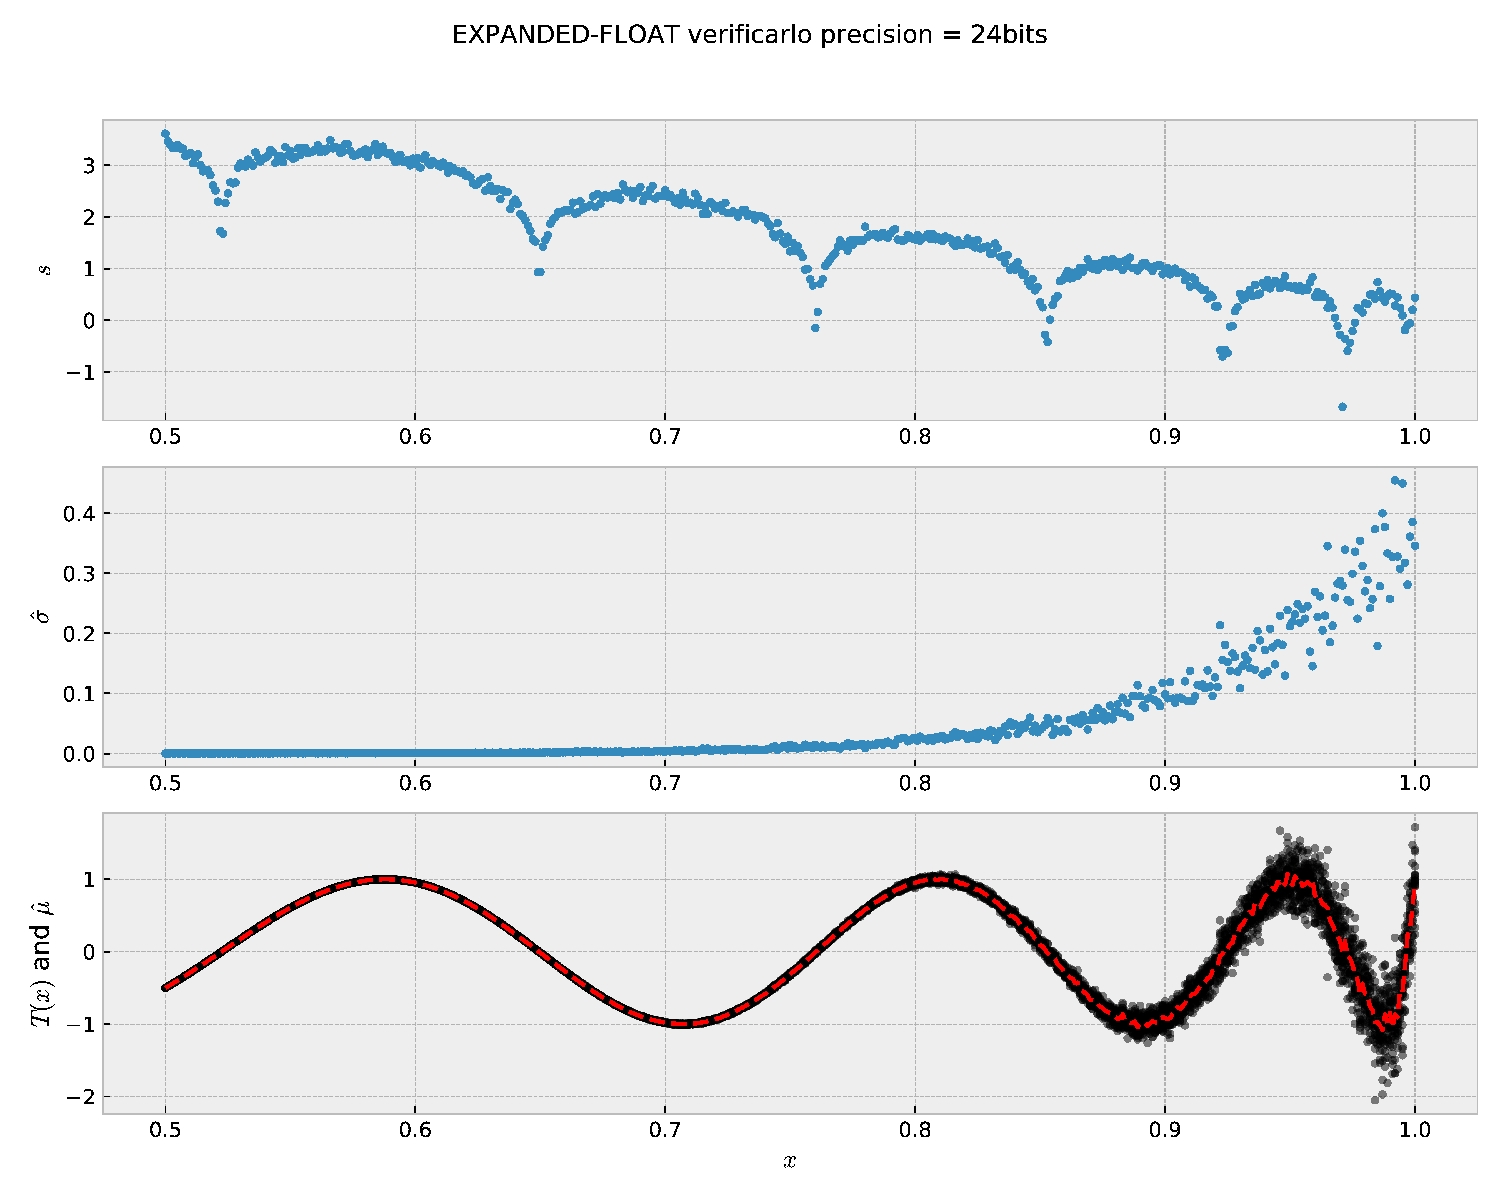
\includegraphics[width=.47\textwidth]{EXPANDED-FLOAT-24.pdf} &
    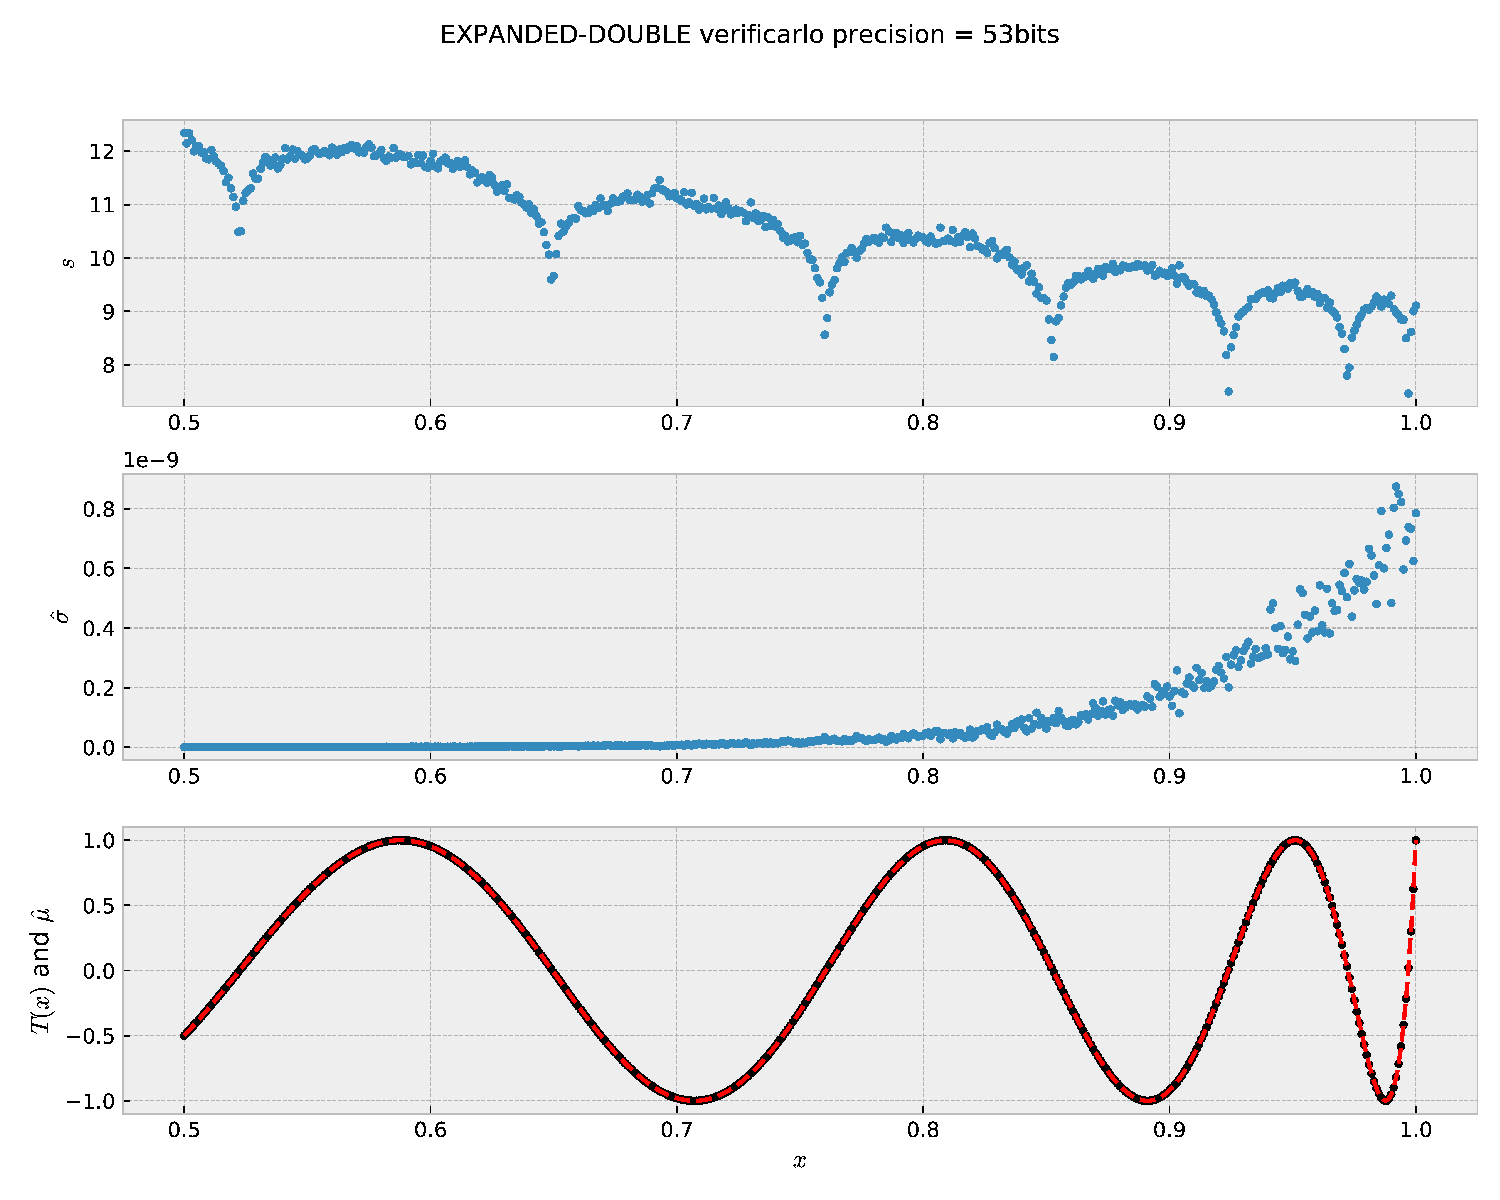
\includegraphics[width=.47\textwidth]{EXPANDED-DOUBLE-53.pdf}  \\
    %Expanded form, 24 bits & Expanded form, 53 bits \\
  \end{tabular}
  \caption{Evaluation of T(x) in Expanded form, compiled in single/double precision, with a virtual precision of 24/53 bits}
  \label{fig:exp_24_53}
\end{table}

The polynomial evaluation done with 24 bits is subject to severe {\it cancellations} when the input value is close to $1$.
This drasticaly reduces the accuracy of the result.
Using evaluation in double precision on the contrary seems satisfactory. But
this solution forces the developer to use a larger and more expensive data type
and it does not solve the problem, it only delays it.

\FloatBarrier



%% Uncomment below lines to include the Factored Form + VPREC
\FloatBarrier
\subsection{Factored form}

We will now evaluate the evaluation precision of the following factored rewriting:
\[
    T(x) = 1 + 8x^2\,(x-1)\,(x+1)\,(4x^2 + 2x - 1)^2\, (4x^2 - 2x - 1)^2\,(16x^4 - 20x^2 + 5)^2
\]

\begin{eqnarray*}
    T(x) &=& 8.0*x^2*(x - 1.0)*(x + 1.0) \\
    & & * (4.0*x^2 + 2.0*x - 1.0)*(4.0*x^2 + 2.0*x - 1.0) \\
    & & * (4.0*x^2 - 2.0*x - 1.0)*(4.0*x^2 - 2.0*x - 1.0)* \\
    & & * (16.0*x^4 - 20.0*x^2 + 5.0)*(16.0*x^4 - 20.0*x^2 + 5.0) + 1 \\
\end{eqnarray*}

\begin{question}
    \begin{enumerate}[(a)]
        \item Open the file {\tt tchebychev.c} and have a look to the function {\tt REAL factored (REAL x)}
        \item Execute the command {\tt ./run.sh FACTORED FLOAT 24} \newline
              The output of this command is given in figure~\ref{fig:factored:float}.
        \item Compare these results to those obtained with the EXPANDED version.
    \end{enumerate}
\end{question}

\begin{figure}[h]
    \center 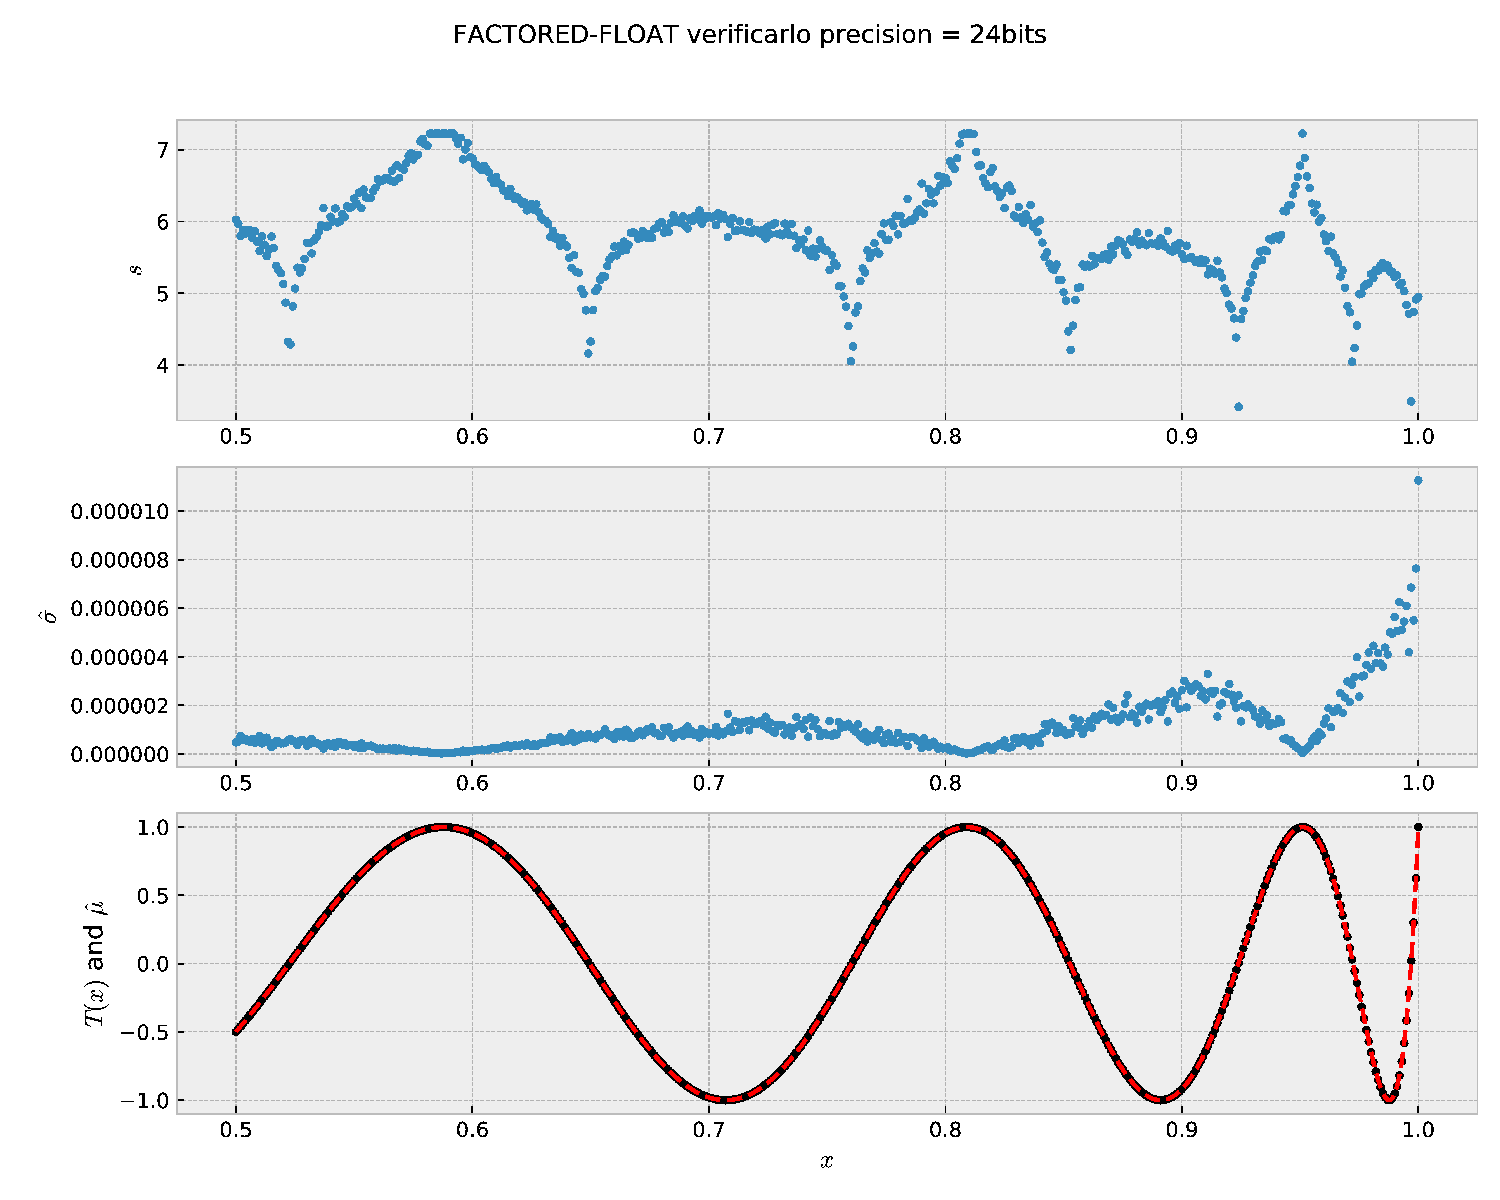
\includegraphics[width=.8\textwidth]{FACTORED-FLOAT-24.pdf}
    \caption{Evaluation of T(x) in its factored form, compiled in single precision, with a virtual precision of 24}
    \label{fig:factored:float}
\end{figure}

\begin{question}
    Explain what happens when $T(x)=1$ for $x\simeq 0.6$,
    $x\simeq 0.8$ et $x\simeq 0.95$.\\~\\
    $\rightarrow$ We evaluate $T$ on one of the roots of the factored right-hand terms which become zero.
    It is an example where the error is absorbed and the precision and accuracy of the results are improved.
\end{question}


%\begin{question}
%  \begin{enumerate}[(a)]
%    \item Modify the {\tt run.sh} script to evaluate the  polynomial between $0.99$ and $1$ by $0.00001$ step.
%    \item Run the scripts to execute and visualize the results for
%          FACTORED, EXPANDED and HORNER with a virtual precision of 53. The results are respectively presented in figure~\ref{fig:factored:double:53:zoom},\ref{fig:expanded:double:53:zoom}
%          and~\ref{fig:horner:double:53:zoom}.
%
%    \item Reproduce the result with a virtual precision of 24. The results are respectively presented in figure~\ref{fig:factored:double:24:zoom},\ref{fig:expanded:double:24:zoom}
%          and~\ref{fig:horner:double:24:zoom}
%
%  \end{enumerate}
%\end{question}
%
%\begin{figure}[h]
%  \center 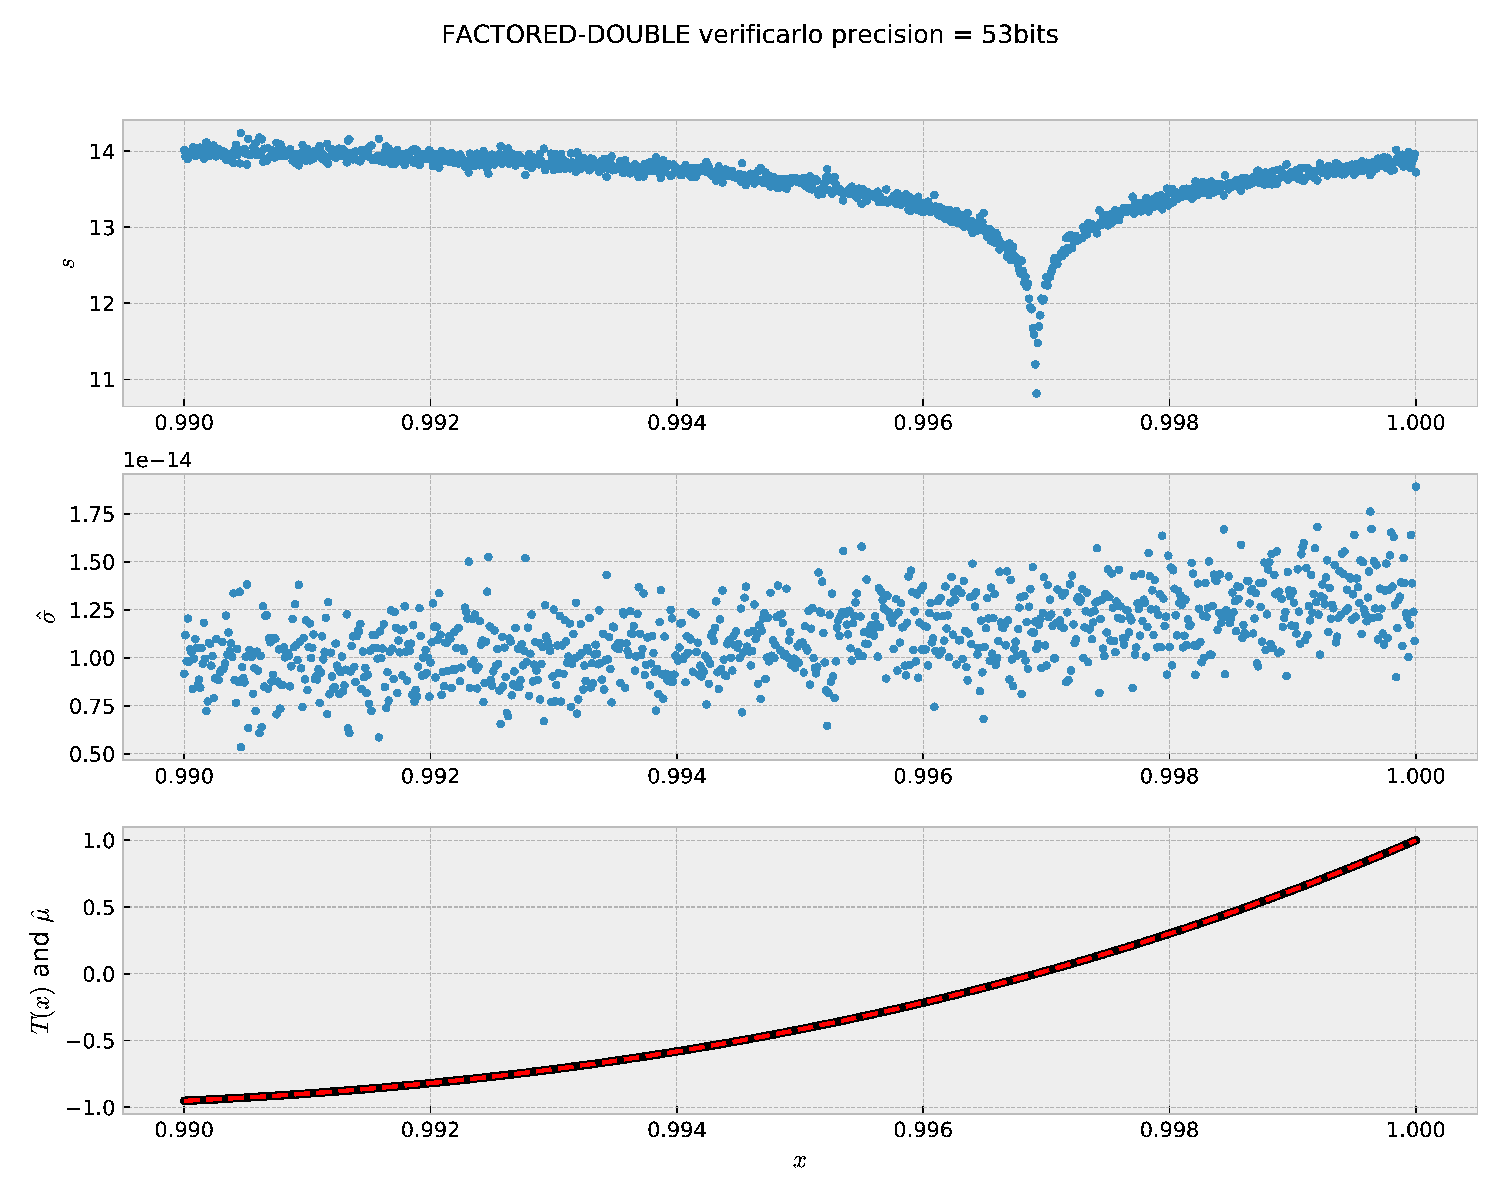
\includegraphics[width=.8\textwidth]{FACTORED-DOUBLE-53-zoom.pdf}
%  \caption{Evaluation of T(x) in its factored form, compiled in double
%    precision, with a virtual precision of 53}
%  \label{fig:factored:double:53:zoom}
%\end{figure}

%\begin{figure}[h]
%  \center 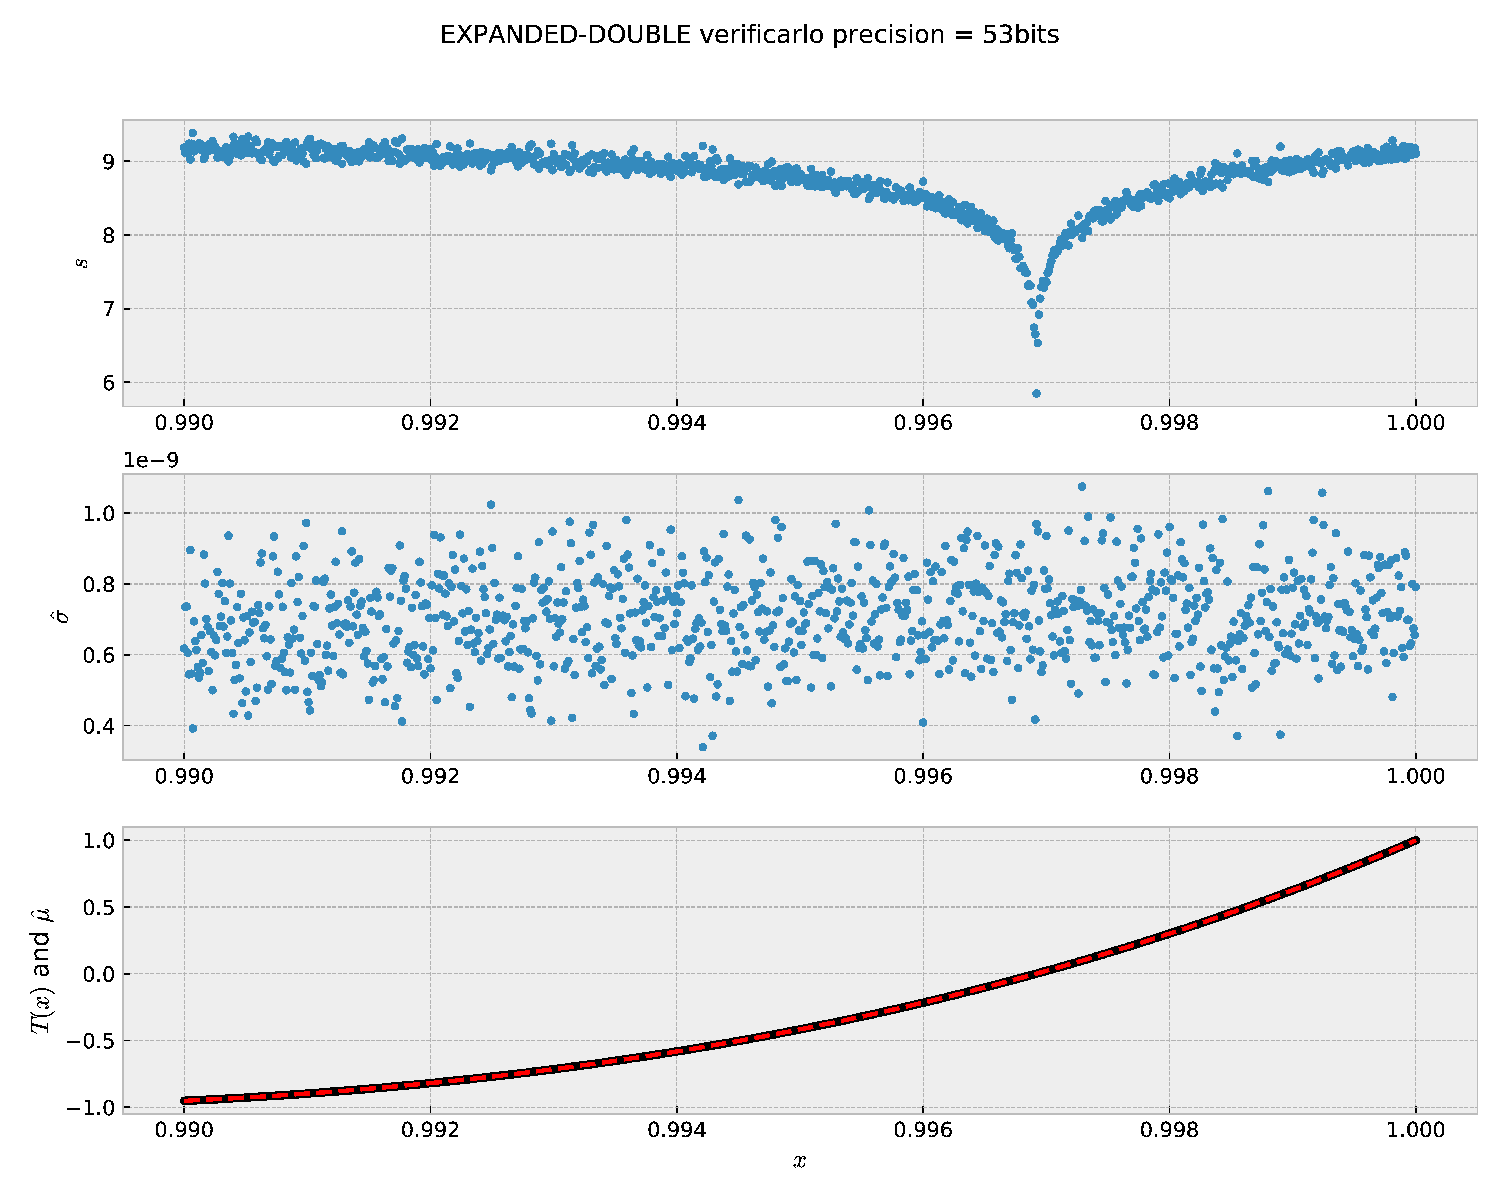
\includegraphics[width=.8\textwidth]{EXPANDED-DOUBLE-53-zoom.pdf}
%  \caption{Evaluation of T(x) in its expanded form, compiled in double
%    precision, with a virtual precision of 53}
%  \label{fig:expanded:double:53:zoom}
%\end{figure}
%
%\begin{figure}[h]
%  \center 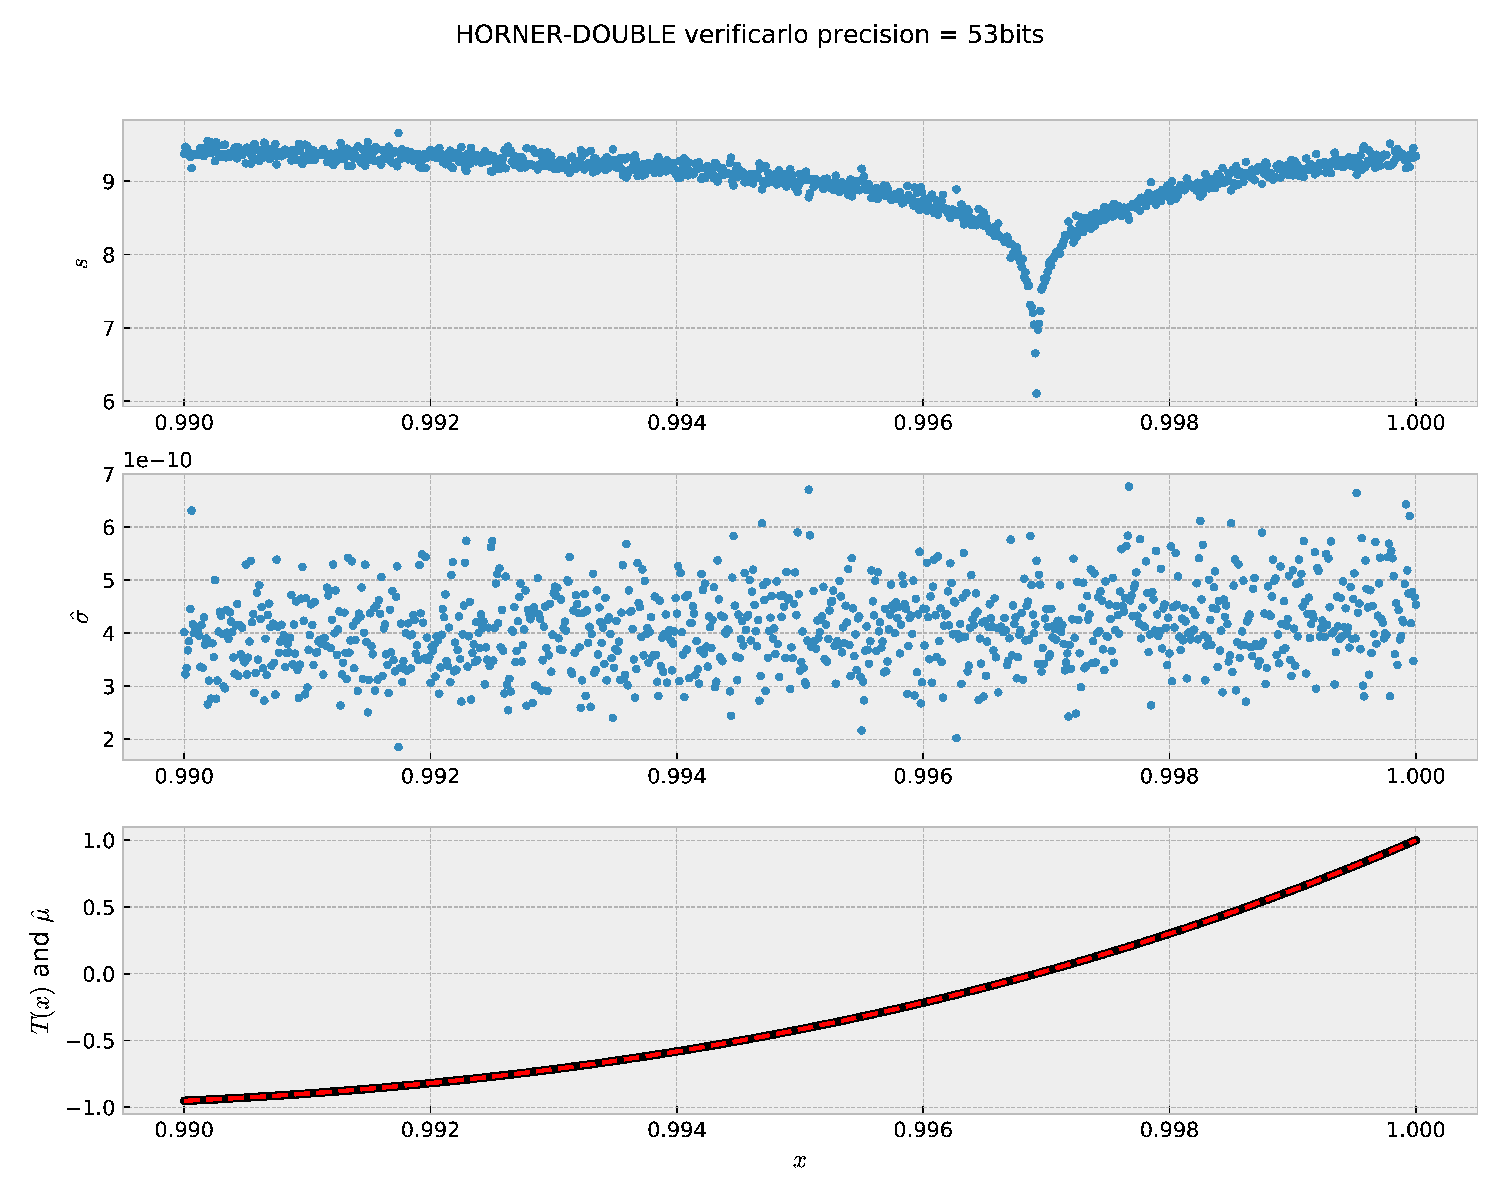
\includegraphics[width=.8\textwidth]{HORNER-DOUBLE-53-zoom.pdf}
%  \caption{Evaluation of T(x) using Horner scheme, compiled in double precision,
%    with a virtual precision of 53}
%  \label{fig:horner:double:53:zoom}
%\end{figure}
%
%\begin{figure}[h]
%  \center 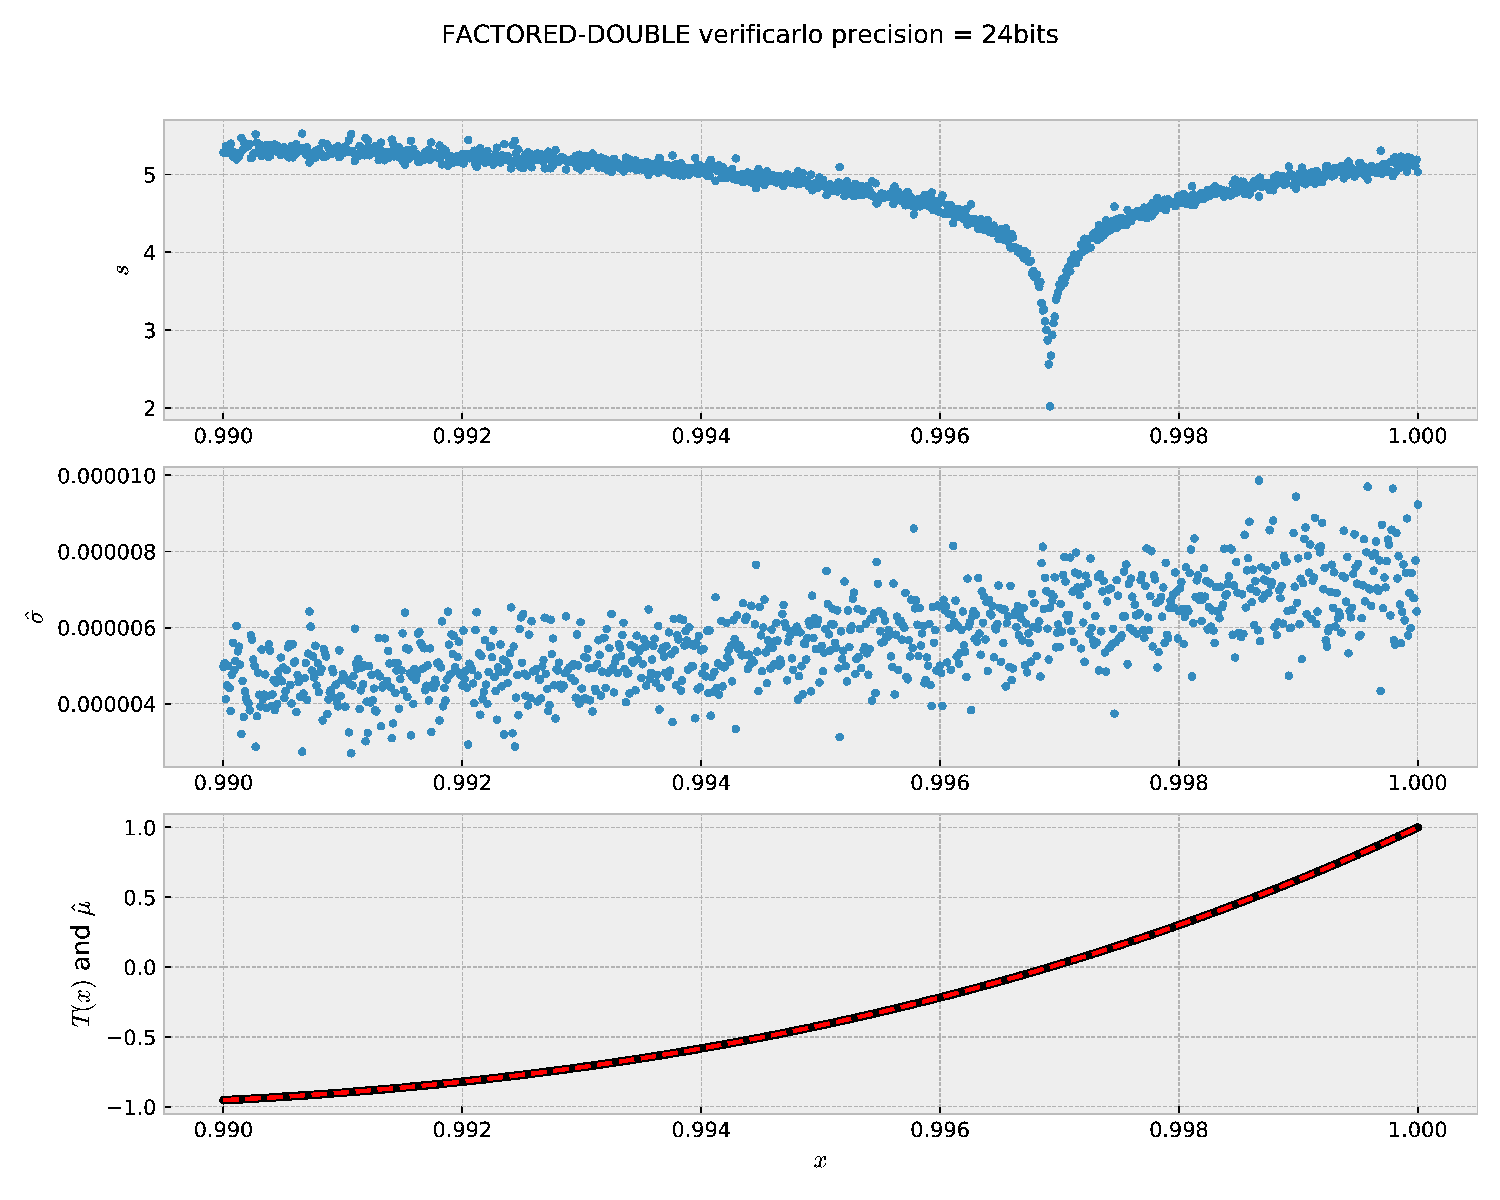
\includegraphics[width=.8\textwidth]{FACTORED-DOUBLE-24-zoom.pdf}
%  \caption{Evaluation of T(x) in its factored form, compiled in double
%    precision, with a virtual precision of 24}
%  \label{fig:factored:double:24:zoom}
%\end{figure}
%
%\begin{figure}[h]
%  \center 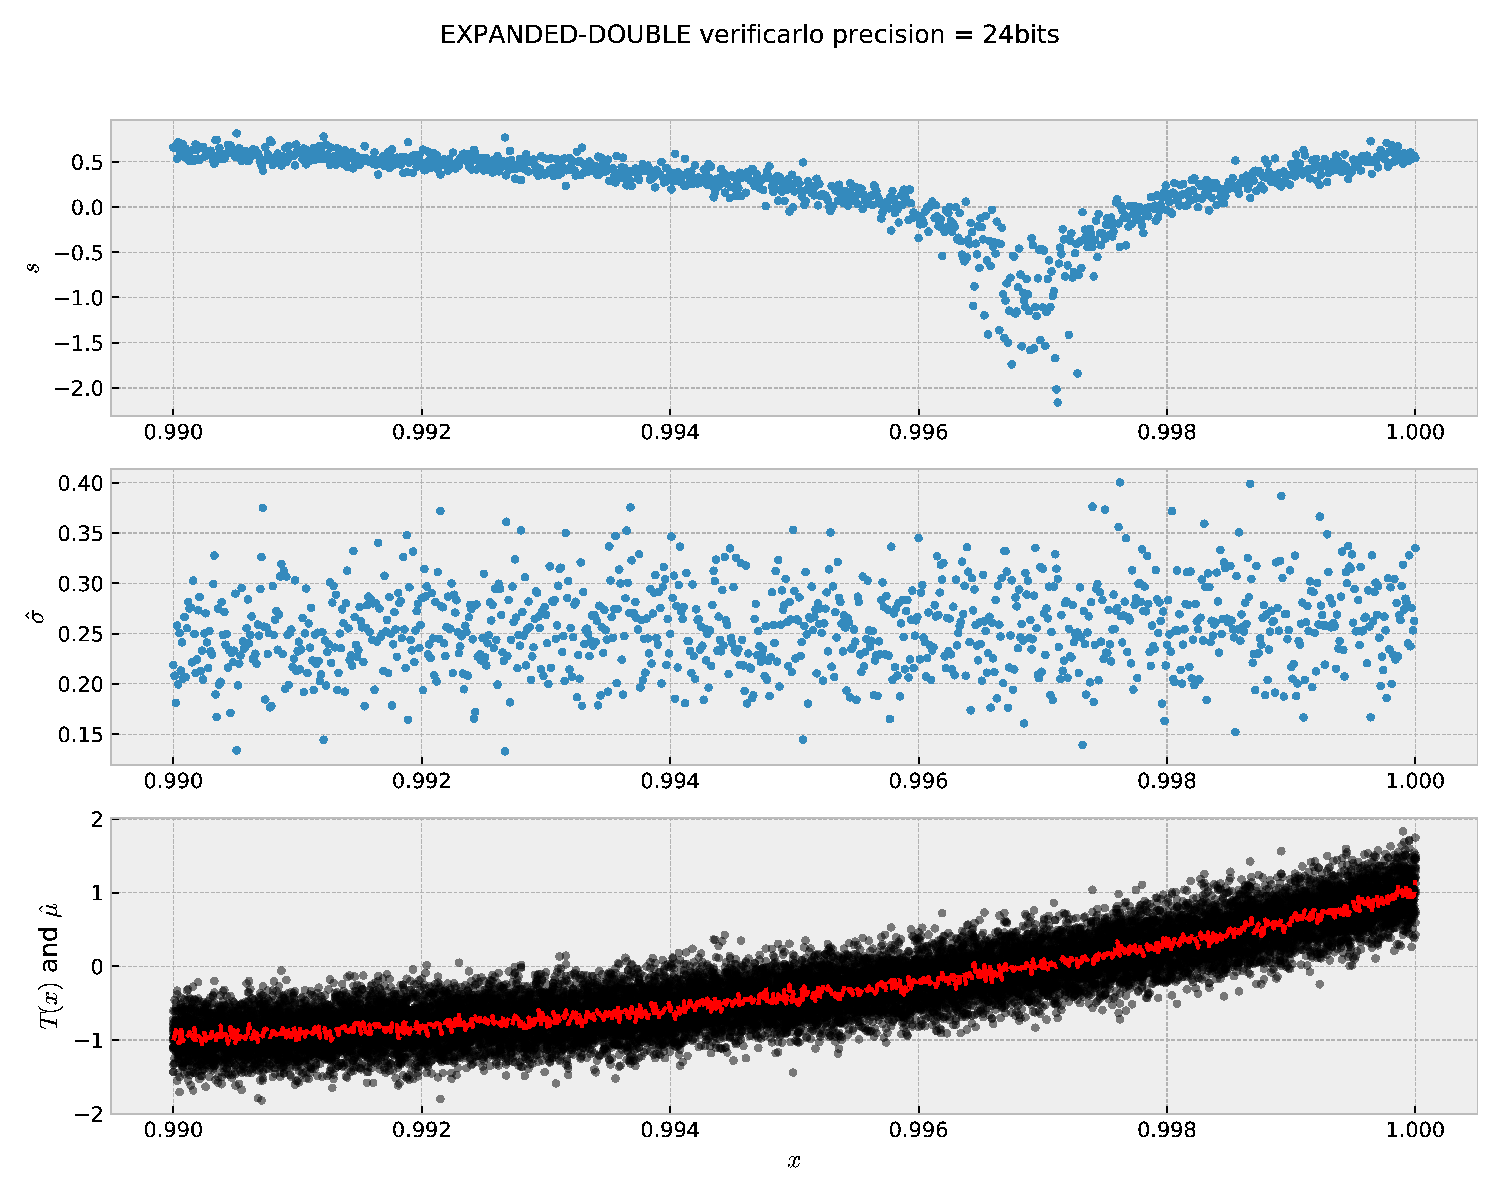
\includegraphics[width=.8\textwidth]{EXPANDED-DOUBLE-24-zoom.pdf}
%  \caption{Evaluation of T(x) in its expanded form, compiled in double
%    precision, with a virtual precision of 24}
%  \label{fig:expanded:double:24:zoom}
%\end{figure}
%
%\begin{figure}[h]
%  \center 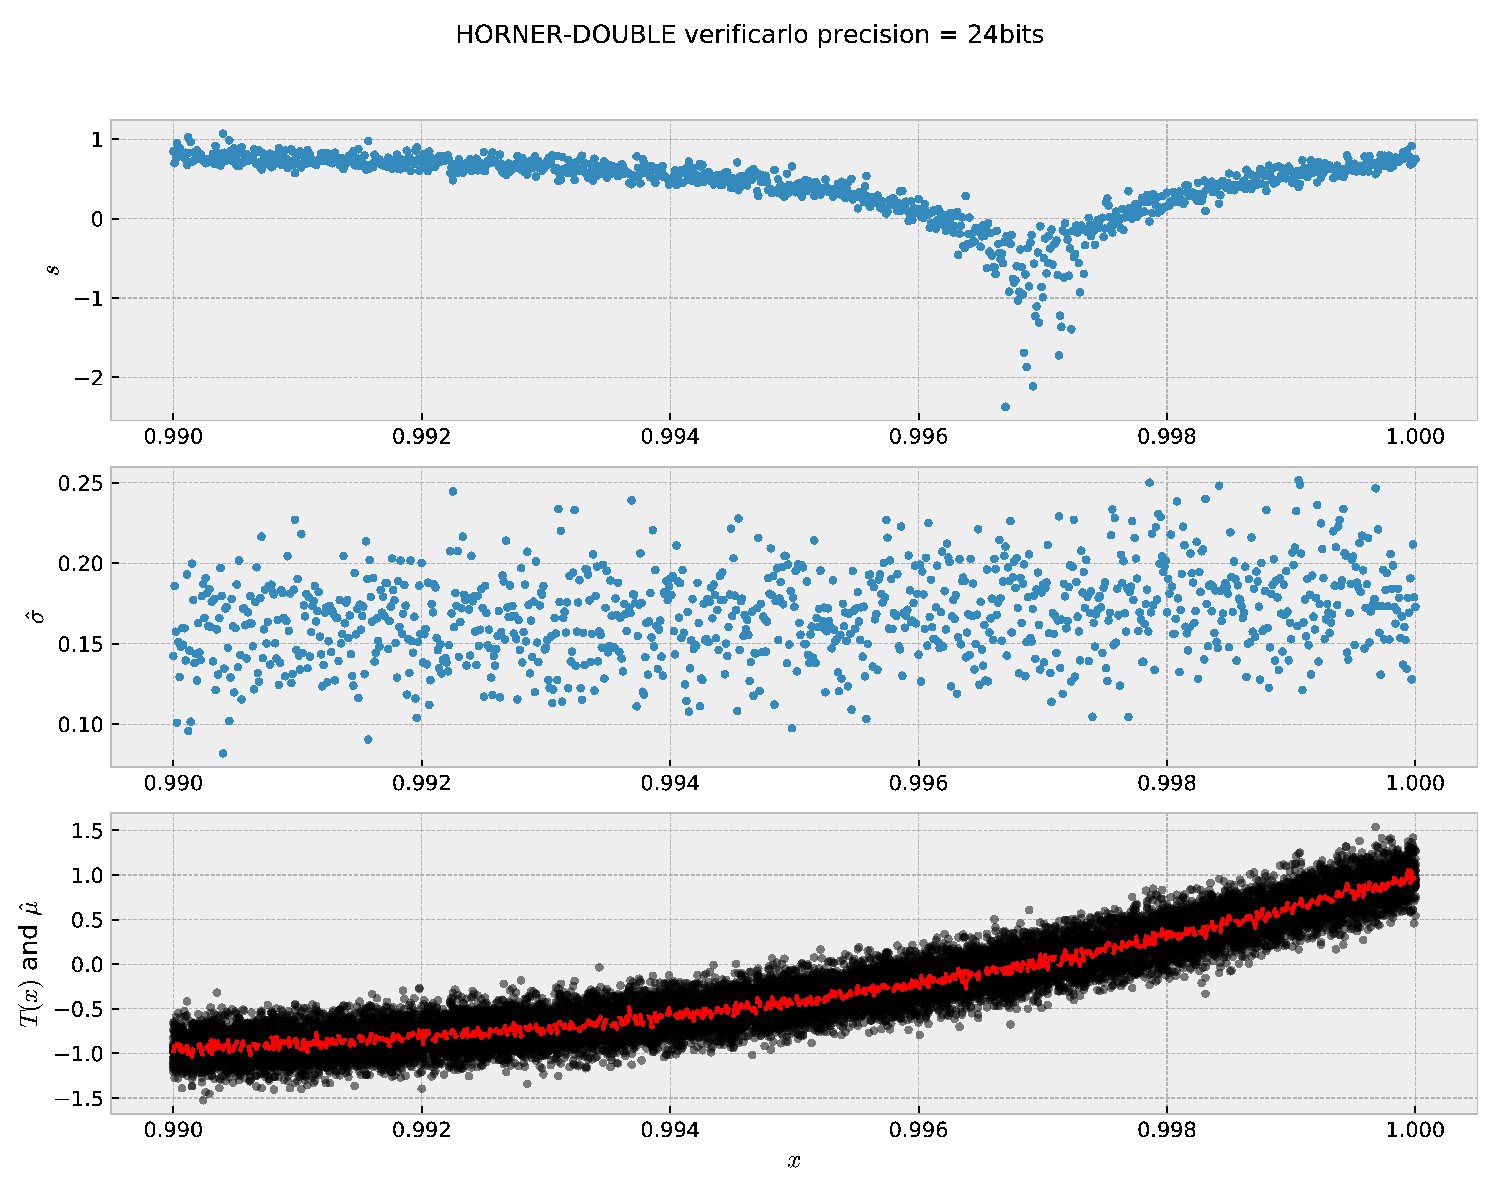
\includegraphics[width=.8\textwidth]{HORNER-DOUBLE-24-zoom.pdf}
%  \caption{Evaluation of T(x) using Horner scheme, compiled in double precision,
%    with a virtual precision of 24}
%  \label{fig:horner:double:24:zoom}
%\end{figure}

\section{VPREC: Variable precision backend}

The VPREC backend emulates reduced floating-point formats without having to
change the implementation. It can emulate any format that fits into the original
type. Unlike the MCA backend, VPREC is deterministic. It mirrors what would happen
with the selected reduced type. It correctly handles overflow, underflows, and
rounding in the target type.

To use VPREC one can either tune manually the range and precision of the target
type. The option {\tt --precision-binary64=PRECISION} controls the
pseudo-mantissa bit length of the new tested format for floating-point
operations in double precision. The option {\tt --range-binary64=PRECISION}
controls the exponent bit length of the target format.

One can also use one of the standard presets: binary16, binary32, bfloat16,
tensorfloat, fp24, PXR24; which automatically sets the corresponding range and
precisions. The option for setting a preset is {\tt --preset=PRESET}.


\begin{question}
    \begin{enumerate}[(a)]
        \item Compile and run the benchmark using single precision without verificarlo
              \begin{verbatim}
clang -D FLOAT -o reference tchebychev.c
./reference 0.6 FACTORED
6.0000002e-01 9.5425093e-01
\end{verbatim}
        \item Now compile it using double precision with verificarlo
              \begin{verbatim}
verificarlo -D DOUBLE -o tchebychev tchebychev.c
VFC_BACKENDS="libinterflop_vprec.so --preset=binary32" ./tchebychev 0.6 FACTORED 
5.9999999999999998e-01 9.5425069332122803e-01
\end{verbatim}
        \item Compare the mantissas between the two previous runs. Observe that VPREC has accurately emulated binary32 (FLOAT) format.
    \end{enumerate}
\end{question}

\begin{question}
    \begin{enumerate}[(a)]
        \item You can emulate the effect of bfloat16 using
              \begin{verbatim}
VFC_BACKENDS="libinterflop_vprec.so --preset=bfloat16" ./tchebychev 0.6 FACTORED 
5.9999999999999998e-01 9.5312500000000000e-01
\end{verbatim}
        \item You can also emulate a custom precision, such as 10 bits, with
              \begin{verbatim}
VFC_BACKENDS="libinterflop_vprec.so --precision-binary64=10" ./tchebychev 0.6 FACTORED 
5.9999999999999998e-01 9.5263671875000000e-01
\end{verbatim}
        \item Try different precisions, at which threshold does the computation looses all significance ?
    \end{enumerate}
\end{question}

\begin{question}
    \begin{enumerate}[(a)]
        \item Analyze the script {\tt run\_vprec.sh}. This script allows you to plot the result of VPREC runs in the interval $[0.5,1]$.
        \item Use the script to simulate and plot the effect of running FACTORED and EXPANDED versions with bfloat16.
    \end{enumerate}
\end{question}


%% Uncomment the following line to include Delta Debug in the tutorial
\FloatBarrier
\section{Pinpointing bugs with Delta-Debug: Archimedes' method}

\begin{figure}[h]
  \centering
  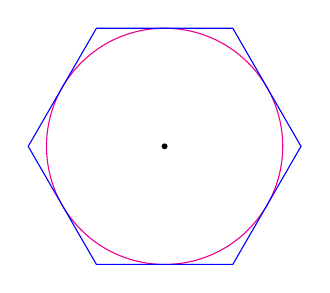
\begin{tikzpicture}[scale=1.5]
    \draw [magenta] (0,0) circle (1);
    \draw [fill, black] (0,0) circle (.02);
    \begin{scope}[yshift=1cm]
    \draw [blue, turtle={ home,
      right=90, forward=.5773502691896257, % tan(pi/6)
      right=60, forward=2*.5773502691896257,
      right=60, forward=2*.5773502691896257,
      right=60, forward=2*.5773502691896257,
      right=60, forward=2*.5773502691896257,
      right=60, forward=2*.5773502691896257,
      right=60, forward=.5773502691896257
    }];
    \end{scope}
\end{tikzpicture}
  \caption{Archimedes method to approximate $\pi$ with a 6-sided circumscribed polygon.
    \label{fig:archimedes}
  }
\end{figure}

In this section we demonstrate how we can use Verificarlo to precisely localize a numerical bug in a program. The localization method is based on the Zeller's Delta-Debug reduction method~\cite{zeller2001automated}. Verificarlo uses the Interflop's stochastic Delta-Debug library developped by Bruno Lathuilière and François Fevotte.

In 200BC Archimedes proposed the first numerical method for computing $\pi$.
Archimedes method uses a $(6.n)$-sided circumscribed polygon to the unit circle
whose area provides an upper bound for $\pi$ and a $(6.n)$-sided inscribed polygon
whose area provides a lower bound for $\pi$.

Here we will use the circumscribed polygon to approximate $\pi$.
Figure~\ref{fig:archimedes} shows a 6-sided circumscribed polygon to the unit
circle. Archimedes shows geometrically that the half-perimeter of the polygons (also converging to $\pi$) can be computed with the following recursive sequence,

\begin{align*}
  T_1 &= \frac{1}{\sqrt{3}} \\
  T_{i+1} &= \frac{\sqrt{T_i^2+1} - 1}{T_i} \\
  \frac{P_{i}}{2} &= 6 \times 2^{i-1} \times T_{i} \xrightarrow[i \to \infty]{} \pi
\end{align*}

In this part of the tutorial we will work inside the \texttt{archimedes/} folder.

\begin{question}
  \begin{enumerate}[(a)]
    \item Open the file \texttt{archimedes.c} and analyze the code.
    \item The provided makefile builds the program using Verificarlo. Run the program
      with the IEEE backend (\texttt{libinterflop\_ieee.so}) and with the MCA backend
      (\texttt{libinterflop\_mca.so -{}-precision 53}).
    \item How many digits are significant in the computed result?
  \end{enumerate}
\end{question}

The previous experiment shows that computation becomes numerically unstable
around iteration 15. Where is the error in the code? To help pinpointing the error,
we are going to use Delta-Debug.

Delta-Debug (DD) is a general bug reduction method that allows to efficiently find a
minimal set of conditions that trigger a bug. In this case, we are going to consider
the set of floating-point instructions in the program. We are using DD to
find a minimal set of instructions responsible for the instability in the output.

\begin{table}[h]
  \centering
  \begin{tabular}{lcr}
    Step & Instructions with MCA noise & Numerically Stable \\
    \midrule
    1    & 1 2 3 4 . . . . & stable \\
    2    & . . . . 5 6 7 8 & unstable \\
    \midrule
    3    & . . . . 5 6 . . & stable \\
    4    & . . . . . . 7 8 & unstable \\
    \midrule
    5    & . . . . . . 7 . & unstable \\
    Result (ddmin) & . . . . . . 7 . & \\
  \end{tabular}
  \caption{Example of Delta-Debug bug minimization\label{tab:deltadebug}}
\end{table}

Table~\ref{tab:deltadebug} shows a simple DD execution to find a reduced
instruction set responsible for a numerical instability. By testing
instructions sub-sets and their complement, DD is able to find smaller failing
sets step by step. DD stops when it finds a failing set where it cannot remove
any instruction. In this case, DD is able to find a minimal failing set (ddmin)
of size 1 (which is therefore also minimum). However, there is no guarantee of unicity.

By default, Interflop's Delta-Debug implementation iterates to find all the
possible different ddmin sets. At the end, it produces the rddmin-cmp set which
is the complement of the union of the ddmin sets. The rddmin-cmp set therefore
includes the "stable" instructions and excludes the "unstable" instructions.

To use Delta-Debug, we need to write two scripts: \begin{itemize}
  \item A first script \texttt{ddRun <output\_dir>}, is responsible for running the program and writing its output inside the \texttt{<output\_dir>} folder.
  \item A second script \texttt{ddCmp <reference\_dir> <current\_dir>}, takes as parameter two folders including respectively the outputs from a reference run and from the current run. The \texttt{ddCmp} script must return with a success when the deviation between the two runs is acceptable, and fail if the deviation is unacceptable.
    To decide if a given set is unstable, DD will run the program five times (the number of times can be changed by setting the environment variable \texttt{INTERFLOP\_DD\_NRUNS}).
\end{itemize}

\begin{question}
  \begin{enumerate}[(a)]
    \item Open the files \texttt{ddRun} and \texttt{ddCmp} and analyze how they work.
  \end{enumerate}
\end{question}

\texttt{ddRun} a \texttt{ddCmp} depend on the user's application and the error tolerance
of the application domain; therefore it is hard to provide a generic script that fits all cases. That is why we require the user to manually write these scripts.
Once the scripts are written, the Delta-Debug session is launched using the following command:

\begin{verbatim}
VFC_BACKENDS="libinterflop_mca.so -p 53 -m mca" vfc_ddebug ddRun ddCmp
\end{verbatim}

where \texttt{VFC\_BACKENDS} specifies the noise model that will be used to
simulate numerical errors. Here we provide a simple Makefile target that
runs this command,
\begin{verbatim}
make dd MCA_MODE="-p 53 -m mca"
\end{verbatim}

\begin{question}
  \begin{enumerate}[(a)]
    \item Open the file \texttt{Makefile} and analyze the \texttt{make dd} target.
    \item Run the \texttt{make dd} target.
  \end{enumerate}
\end{question}

Now that you have run Delta-Debug, you can observe that it has found two minimal failing sets (ddmin0 and ddmin1). The outputs sets are located in \texttt{dd.line/ddmin0} and \texttt{dd.line/ddmin1} directory. You can locate the "unstable" instructions belonging to each set by browsing the content of the \texttt{dd.line/ddmin{0,1}/dd.line.include} files. This information is also present in the \texttt{dd.line/rddmin-cmp/dd.line.exclude} file.

\begin{verbatim}
$ cat dd.line/ddmin0/dd.line.include
0x0000000000400e5c: archimedes at archimedes.c:16
$ cat dd.line/ddmin1/dd.line.include
0x0000000000400e89: archimedes at archimedes.c:17

# We can also get the union of culprit instructions with

$ cat dd.line/rddmin-cmp/dd.line.exclude
0x0000000000400e5c: archimedes at archimedes.c:16
0x0000000000400e89: archimedes at archimedes.c:17
\end{verbatim}

We can notice that instructions at line 16 and 17 found by DD method are responsible for the observed numerical instability. To ease the debugging process we include a script that transforms this output, into the error format used by compilers. Therefore we can use a standard IDE to pinpoint culprit instructions inside the code.

\begin{question}
  \begin{enumerate}[(a)]
    \item Run the \texttt{make dderrors} target. This should open a Vim session.
    \item Type \texttt{:cw} to open the error quick-fix window. Use \texttt{:cn} and \texttt{:cp} to move to the next and previous "unstable" instructions.
  \end{enumerate}
\end{question}

Line 17 points to a subtraction operation executed in double precision (doublesub) between $s$ and $1$. One can see that as $T_{i+1}$ (\texttt{tii}) becomes smaller, $s$ becomes closer to $1$. Therefore it looks like line 17 could trigger a catastrophic cancellation.
Let us do some experiments to confirm this hypothesis.

\begin{question}
  \begin{enumerate}[(a)]
    \item Run Delta-Debug with a RR noise model at precision 53.
      \begin{verbatim}
make dd MCA_MODE="-m rr -p 53"
      \end{verbatim}
  \end{enumerate}
\end{question}

With RR 53, only line 16 is flagged. Indeed the operation $T_i^2+1$ is inexact
due to a round-off error ($T_i \ll 1$). The error then propagates and is amplified
by the cancellation line 17.

Interestingly, with RR the line 17 is not flagged; that is because RR 53 mode
does not perturb cancellations which are exact operations. The fact that line
17 disappears with RR mode hints that there is indeed a cancellation problem.

\begin{question}
  \begin{enumerate}[(a)]
    \item Run Delta-Debug with a PB noise model at precision 53.
      \begin{verbatim}
make dd MCA_MODE="-m pb -p 53"
      \end{verbatim}
  \end{enumerate}
\end{question}

With PB noise model we see again that both line 16 and 17 are flagged.
Therefore, we conclude that this program is affected both by a round-off error
at line 16 and a cancellation error at line 17. The round-off error by itself
is not problematic but is amplified by the cancellation.

To fix this problem, we can try to rewrite the culprit expression in line 17.
Observe that,

\begin{align*}
  T_{i+1} &= \frac{\sqrt{T_i^2+1} - 1}{T_i} = \frac{\sqrt{T_i^2+1} - 1}{T_i} \times \frac{\sqrt{T_i^2+1} + 1}{\sqrt{T_i^2+1} + 1} \\
          &= \frac{(T_i^2 + 1) - 1}{T_i(\sqrt{T_i^2+1} + 1)} \\
          &= \frac{T_i}{\sqrt{T_i^2+1} + 1}
\end{align*}

The new formula is interesting since it eliminates the subtraction that triggered the cancellation.

\begin{question}
  \begin{enumerate}[(a)]
    \item Modify \texttt{archimedes.c} to use the previous expression rewriting.
    \item Study the numerical instability of the new version. Is the problem fixed?
  \end{enumerate}
\end{question}


%% Uncomment below lines to include the extra Horn Compensated analysis
\FloatBarrier
\subsection{BONUS: Compensated Horner's method}
This section corresponds to a Bonus exercice on the Compensated Horner's Method.

"Compensated" algorithms belong to the class of algorithms that increase
program precision without changing the internal working format.
The goal is to capture for each operation an estimation of the error term and to reinject it into the result.
For the Horner scheme, it is possible to retrieve at every step the error in
$x^2$ and the addition of the next coefficient by using respectively the
$Veltkamp-Dekker$ {\tt TWOPROD} for the product and { \tt TWOSUM } for the sum.
These algorithms are qualified as ({\it Error Free Transform}), EFT, in the
literature.
The algorithm for the compensated horner scheme described in \cite{graillat2005compensated} is:

\begin{algorithmic}[1]
  \Procedure{compHorner}{$x$,$\{a_1, a_2, \ldots, a_n\}$}
    \State {$s_n \gets a_n$}
    \State {$r_n \gets 0$}
    \For {$i \in [n-1:0]$}
       \State $[p_i, pe_i] \gets \text{\sc TWOPROD}(s_{i+1}, x^2)$
       \State $[s_i, se_i] \gets \text{\sc TWOSUM}(p_i, a_i)$
       \State $r_i \gets r_{i+1}\times x^2+(pe_i+se_i)$
    \EndFor
    \State \Return $s_0 + r_0$
  \EndProcedure
\end{algorithmic}

The lines 5 and 6, evaluate HORNER with EFT calls. Line 7 accumulates the error terms, which will be added to the final result in line 9.

We provide implementations for EFT in the {\tt libeft.c} and {\tt libeft.h} files.

\begin{question}
  \begin{enumerate}[(a)]
    \item Implement comphorner algorithm in {\tt tchebychev.c} using the EFT implementations in {\tt eft.h}.
    \item Modify {\tt run.sh} to also compile eft.c with verificarlo.
    \item Run comphorner with the following command: {\tt ./run.sh COMPHORNER FLOAT 24 rr}
    \item Run comphorner with the following command: {\tt ./run.sh COMPHORNER DOUBLE 53 rr}
    \item What happens if you use a precision different from 53 for program compiled in DOUBLE precision?
      $\Rightarrow$ WARNING, {\sc TWOPROD} and {\sc TWOSUM} rely on exact operations; it is essential to use RR 53 (Random Rounding with precision 53) mode of verificarlo for  \texttt{double} or RR 24 for \texttt{float}.
      \\~\\
      You should get the results in table~\ref{fig:comphornerVerificarlo24_53}.

  \end{enumerate}
\end{question}


\begin{table}
\begin{tabular}{cc}
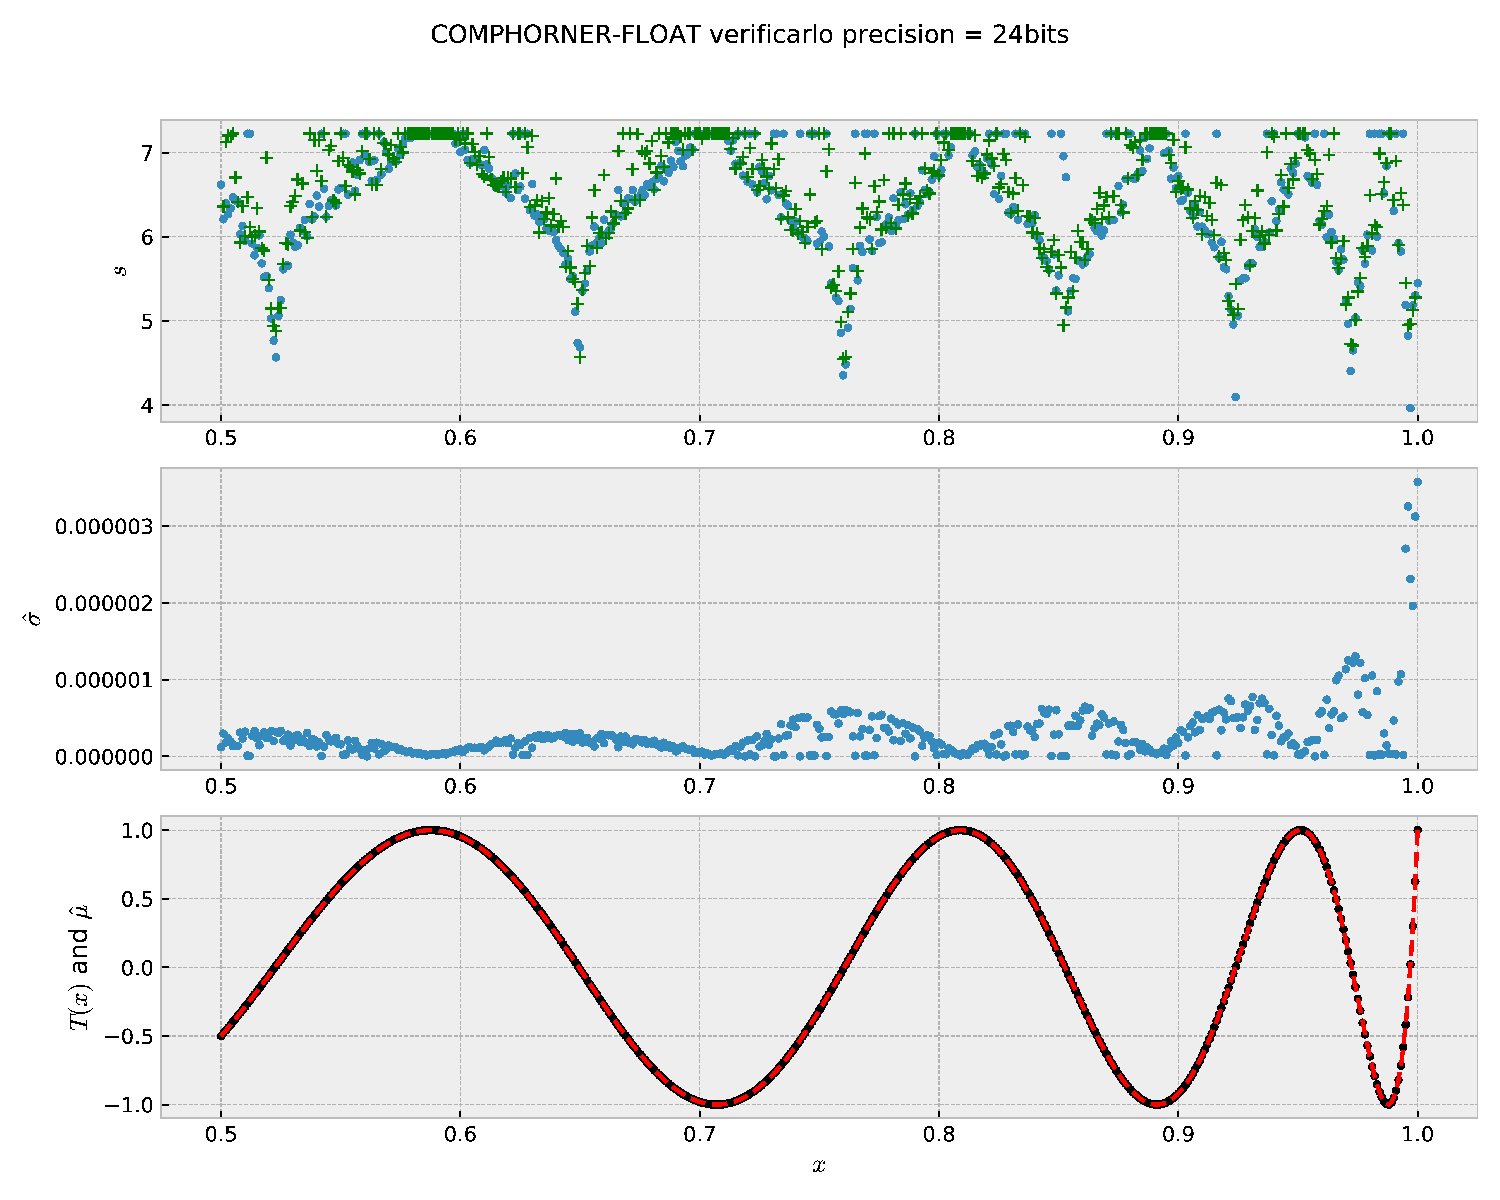
\includegraphics[width=.47\textwidth]{COMPHORNER-FLOAT-24+err.pdf}& 
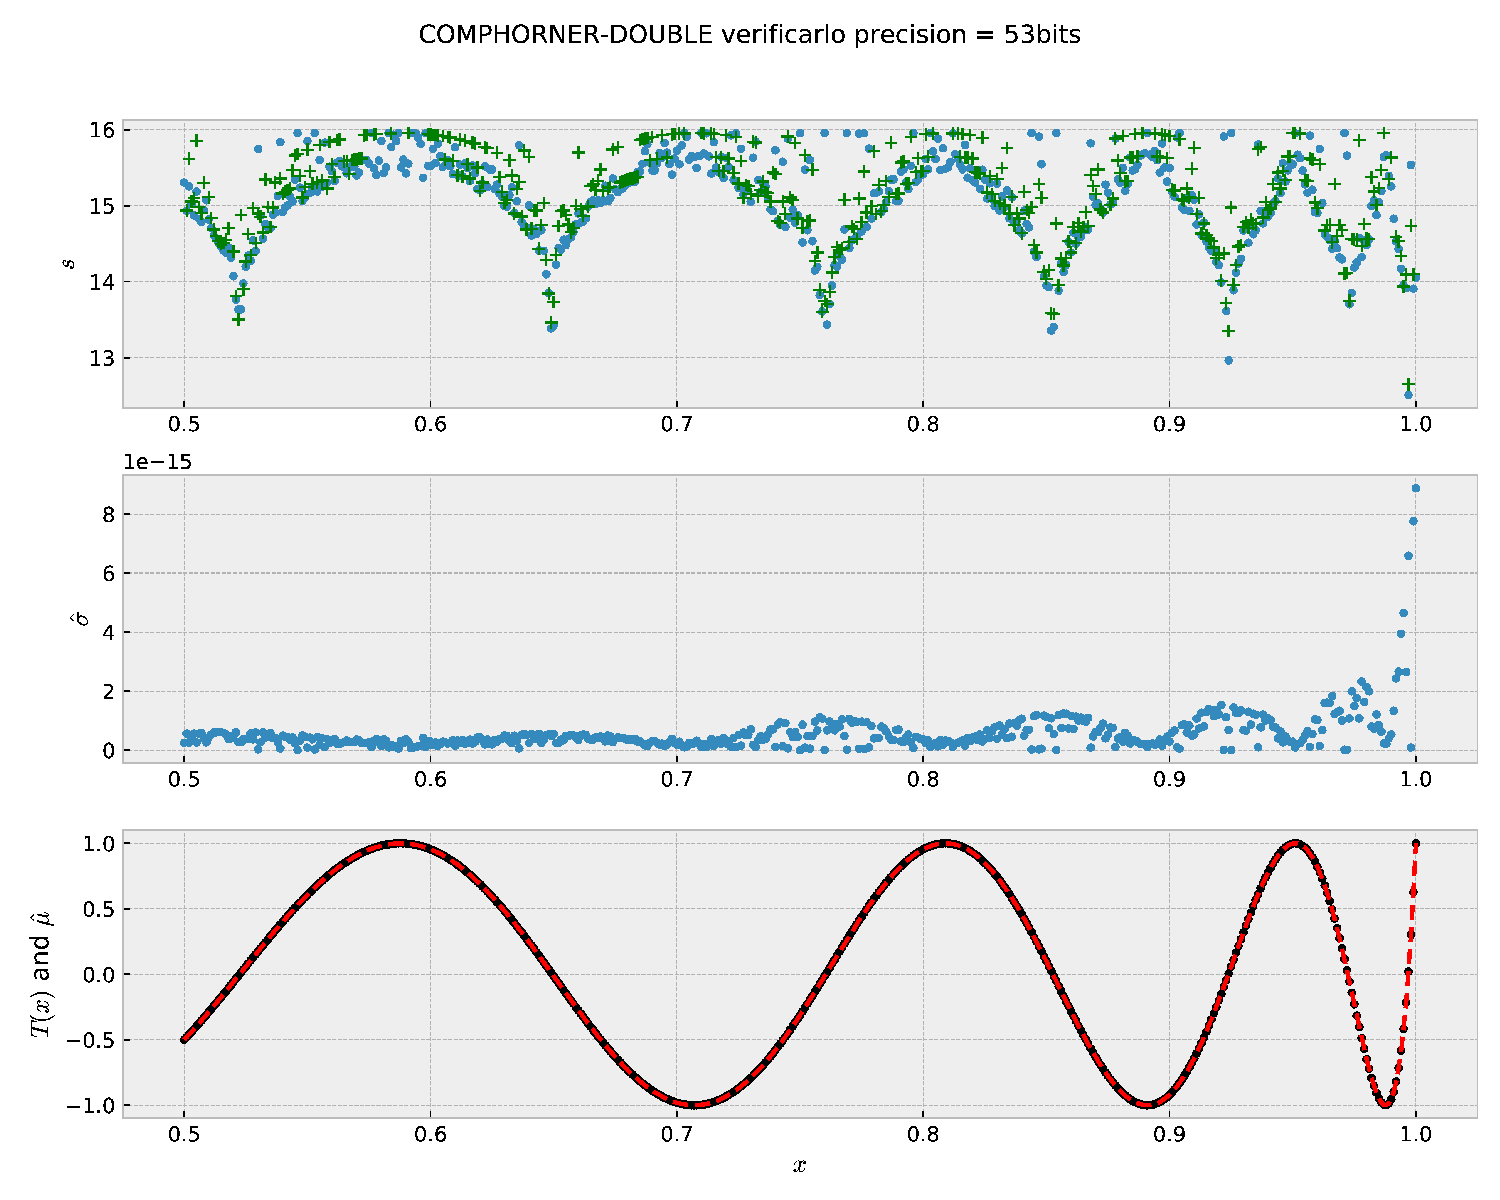
\includegraphics[width=.47\textwidth]{COMPHORNER-DOUBLE-53+err.pdf}\\
\end{tabular}
  \caption{Evaluation of T(x) using Horner and compHorner in single/double (left/right) precision: error estimated by verificarlo (blue), compared to the real error (green)}
  \label{fig:comphornerVerificarlo24_53}
\end{table}


The resulting precision of this approach is shown in table~\ref{fig:comphornerVerificarlo24_53} with verificarlo.
Filled circles represent the real error value (evaluating in rational arithmetic in Python); circles represent the quality of the result computed in Monte Carlo Arithmetic with Verificarlo~\cite{verrou}.

We can notice on these figures that CompHorner compensate precision losses in double and single precision. We retrieve a behavior similar to the factored form, in particularly for points $T(x)=1$. However, knowing the polynomial's roots for using the Horner scheme is not required.

Out of these plots, we can make two interesting observations.
First, at the cost of an increasing number of operations, (but generally in the same complexity class) it is possible to recover a part (or the full) precision losses. There are algorithms called "accurate" that compute result without loss of precision, by, for example, recursively keeping errors terms until they can not be represented in the final result and such that rounding is correct ({\it e.g.} $accSum$ of S. Rump).

Second, some algorithms, especially in mathematical libraries (libmath, Intel MKL, Intel VML, libeft) used particularity of the floating-point format. By using Monte Carlo Arithmetic, it can be difficult even impossible to analyze them. In the random rounding specific case (as implemented by verificarlo RR mode with a precision equal to length(mantissa)+1), a large amount of compensated algorithms can be analyzed (including compHorner as seen before). In addition, by their design, these algorithms have a proof of their level's precision correctness, which makes their evaluation by empirical methods useless.


%% Uncomment the following line to include Veritracer in the tutorial
%% \FloatBarrier
%% \input{veritracer}

\FloatBarrier
\newpage
\bibliographystyle{ieeetr}
\bibliography{bibliography}

\end{document}
